\section{Three-Valued Configurations}

A \emph{program configuration} encodes a global state of a program
which consists of (i)~a global store, (ii)~the program-location of
every thread, and (iii)~the status of locks and threads, e.g., if
a thread is waiting for a lock. Technically, we use first-order
logic with transitive-closure to express configurations and their
properties in a parametric way. Formally, we assume that there is
a set of predicate symbols $P$ for every analyzed program each
with a fixed arity. For example, \tableref{Predicates} contains
predicates for partial semantics of Java. The predicates above the
double-line separator are internal $\tvmc$ predicates. The
predicates below the separator are defined by the user who wishes
to capture the thread-semantics of Java.

\begin{itemize}
\item The unary predicate $\isthread(t)$ is used to denote the
objects that are threads. (e.g., in Java - instances of a subclass
of \texttt{class Thread}).
\item For every potential program-location (program label) $lab$ of
a thread $t$, there is a unary predicate $at[lab](t)$ which is
true when $t$ is at $lab$. These predicates will be referred to as
\emph{location predicates}.
\item For every class field and function
parameter \texttt{fld}, a binary predicate $rvalue[fld](o_1,o_2)$
records the fact that the \texttt{fld} of the object $o_1$
pointing to the object $o_2$.
\item The predicates $held\_by(l,t)$, $blocked(t,l)$ and $waiting(t,l)$
model possible relationships between locks and threads.
%\item The predicate $held\_by(l,t)$ is true when the lock $l$
%is acquired by the thread $t$, via a successful
%\texttt{synchronized} statement.
%\item The predicate $blocked(t,l)$ is true when the thread $t$ is
%blocked on the lock $l$, as a result of an unsuccessful
% \texttt{synchronized} statement.
%\item The predicate $waiting(t,l)$ is true when the thread $t$
%is waiting for the lock $l$ as a result of invoking a
%\texttt{wait()} call.
%\item The predicate $idlt(l_1,l_2)$ is used to record a
%partial order between objects. Each object is assumed to have a
%unique id. The predicate $idlt(l_1,l_2)$ is true when the id of
%$l_1$ is less than the id of $l_2$. The order between objects can
%be used for deadlock prevention by breaking cyclic allocation
%requests \cite{IB-D943023}. In Section~\ref{Se:ResourceOrdering}
%we show how our technique can be used to verify that a program
%uses such a resource-allocation policy.
\end{itemize}


Configurations are depicted as directed graphs. Each individual
from the universe is displayed as a node. A unary predicate $p$
which holds for an individual (node) $u$ is drawn inside the node
$u$. The name of a node is written inside angle brackets. Node
names are only used for ease of presentation and do not affect the
analysis. A true binary predicate $p(u_1,u_2)$ is drawn as
directed edge from $u_1$ to $u_2$ labeled with the predicate
symbol. \figref{Concrete} shows a configuration which consists of
4 threads competing for an exclusive shared resource.

\begin{figure*}
\begin{center}
\framebox{
    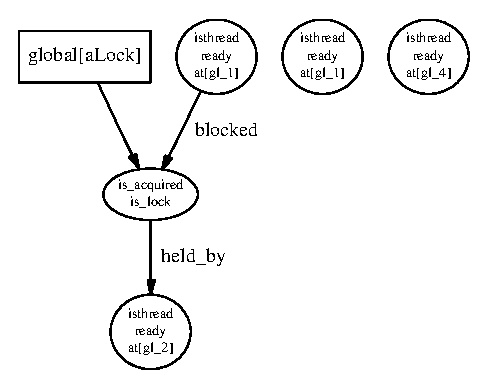
\epsfig{file=figures/concrete,width=3in} %width=4.8in
}
\end{center}
\caption{\label{Fi:Concrete}A concrete configuration
$\C{C_{\ref{Fi:Concrete}}}$.}
\end{figure*}




\begin{table}
\begin{center}
\begin{tabular}{|l|l|} \hline
  % after \\ : \hline or \cline{col1-col2} \cline{col3-col4} ...
  \textbf{Predicates} & \textbf{Intended Meaning} \\
  \hline \hline
  $\isthread(t)$ & \begin{tabular}{l} $t$ is a thread \end{tabular}\\
  \hline
  $\ready(t)$ & \begin{tabular}{l} $t$ is ready for scheduling \end{tabular}\\
  \hline
  $\begin{array}{l}
  \{ at[lab](t) : \\
  ~~~lab \in Labels \}
  \end{array}$ & \begin{tabular}{l} thread $t$ is at label $lab$ \end{tabular} \\
  \hline
  \hline
  $\begin{array}{l}
  \{ rvalue[fld](o_1,o_2) : \\
  ~~~fld \in Fields \}
  \end{array}$ &
  \begin{tabular}{l}
    field $fld$ of the object $o_1$ \\
    points to the object $o_2$ \\
  \end{tabular} \\
  \hline
  $held\_by(l,t)$ & \begin{tabular}{l} the lock $l$ is held by \\ the thread $t$\\
  \end{tabular} \\
  \hline
  $blocked(t,l)$ & \begin{tabular}{l} the thread $t$ is blocked \\ on the lock $l$\\
  \end{tabular} \\
  \hline
  $waiting(t,l)$ &
  \begin{tabular}{l} the thread $t$ is waiting \\ on the lock $l$\\
  \end{tabular} \\
  \hline
  %$idlt(l_1,l_2)$ &
%  \begin{tabular}{l}
%  the id of lock $l_1$ is \\
%  less than the id of lock $l_2$ \\
%  \end{tabular} \\
%  \hline
  %%$runnable(t)$ & is thread $t$ scheduled to execute ? \\
  %%\hline
\end{tabular}
\end{center}
\caption{\label{Ta:Predicates}Predicates for partial Java
semantics.}
\end{table}

$\tvmc$ conservatively represent multiple configurations using a
single logical structure but with an extra truth-value $1/2$
denoting values which may be $1$ and may be $0$. The values $0$
and $1$ are called \emph{definite values} where the value $1/2$
is called \emph{indefinite value}.
